% This is samplepaper.tex, a sample chapter demonstrating the
% LLNCS macro package for Springer Computer Science proceedings;
% Version 2.21 of 2022/01/12
%
\documentclass[runningheads]{llncs}
%
\usepackage[T1]{fontenc}
% T1 fonts will be used to generate the final print and online PDFs,
% so please use T1 fonts in your manuscript whenever possible.
% Other font encodings may result in incorrect characters.
%
\usepackage{graphicx}
% Used for displaying a sample figure. If possible, figure files should
% be included in EPS format.
%
% If you use the hyperref package, please uncomment the following two lines
% to display URLs in blue roman font according to Springer's eBook style:
%\usepackage{color}
%\renewcommand\UrlFont{\color{blue}\rmfamily}
%\urlstyle{rm}
%
\begin{document}
%
\title{ECG Categorization performance with Signal Decomposition and Machine Learning Techniques}
%
%\titlerunning{Abbreviated paper title}
% If the paper title is too long for the running head, you can set
% an abbreviated paper title here
%
\author{Juan Emilio de la Torre Bárcenas\inst{1}\orcidID{A01708606} \and
{Israel Vidal Paredes}\inst{1}\orcidID{A01750543} \and
{Ivan Serrano González}\inst{1}\orcidID{A01748517} \and {Samuel García} \inst{1}\orcidID{A01642317}}
%
\authorrunning{Ivan et al.}
% First names are abbreviated in the running head.
% If there are more than two authors, 'et al.' is used.
%
\institute{Tecnológico de Monterrey Campus Guadalajara, Av. Gral Ramón Corona No 2514, Colonia Nuevo México, 45201 Zapopan, Jal., MEX \\
\url{https://tec.mx/es/guadalajara}}
%
\maketitle              % typeset the header of the contribution
%
\begin{abstract}

This study examines the effectiveness of machine learning algorithms in classifying electrocardiographic (ECG) signal patterns for myocardial infarction (MI) diagnosis. We compare Support Vector Classification (SVC), Random Forest Classification, and Decision Tree Classification on ECG datasets, focusing on optimizing recall performance for accurate MI detection. Additionally, we investigate the impact of signal preprocessing techniques, including Fourier Transform and second derivative analysis, on model performance. Contrary to expectations, our results suggest that these preprocessing methods do not significantly enhance the performance of the mentioned classifiers for ECG signal pattern recognition compared to unprocessed signals. This research contributes to the development of more reliable automated systems for ECG interpretation, potentially reducing misdiagnosis risks and improving patient care outcomes in cardiovascular disease management.

\end{abstract}
%
%
%
\section{Introduction}

\subsection{Motivation for Work}

Myocardial infarction (MI), commonly known as a heart attack, poses a significant global health challenge, representing a leading cause of mortality worldwide. The devastating impact of MI underscores the critical need for timely and accurate diagnosis, enabling prompt intervention and potentially lifesaving treatment. Electrocardiograms (ECGs), which record the electrical activity of the heart, are indispensable tools in the diagnosis of MI and other cardiac conditions. However, the interpretation of ECG signals can be complex and prone to human error, especially in situations where subtle abnormalities are present.


\subsection{Objectives}

This research investigation aims to examine the effectiveness of various machine learning methodologies in classifying electrocardiographic (ECG) signal patterns. The primary focus of this study will be to evaluate the performance of Support Vector Classification (SVC), Random Forest Classification, and Decision Tree Classification algorithms for this purpose.

To achieve this objective, the proposed research will entail:
\begin{enumerate}
    \item Acquisition and preparation of a suitable ECG dataset
    \item Implementation and training of the aforementioned classification models
    \item Comparative analysis of the models' predictive accuracy, precision, and recall rates
    \item Emphasis on optimizing recall performance, given the critical nature of accurately identifying potentially harmful diagnostic outcomes
\end{enumerate}

Furthermore, this study aims to investigate the impact of signal preprocessing techniques on model performance. Specifically, we will compare the effectiveness of the aforementioned machine learning models when trained on:

\begin{enumerate}
    \item The original ECG signal: This baseline will serve as a benchmark for comparison.
    \item Fourier Transform decomposition of frequencies and phase shift: Exploring frequency domain features may enhance the models' ability to distinguish between ECG categories.
    \item Second derivative of the ECG signal: Examining the rate of change in the signal can potentially reveal crucial information for classification.
\end{enumerate}


\subsection{Thesis Statement}
Contrary to prevailing assumptions, this study contends that the application of Fourier Transform and second derivative preprocessing techniques does not yield significant improvements in machine any of the machine learning classifiers' performance for electrocardiographic signal pattern recognition compared to unprocessed signals.
    
\section{Methodology}

\subsection{Dataset}

The dataset consists of a series of signals obtained from an ECG, labeled from 0 to 4 corresponding to each ailment, where 0 corresponds to a Normal category and 1 to 4 an ailment

As outlined by Kauchee et al. \cite{kachuee2018ecg} in their paper, the dataset which was originally obtained from the PhysioNet MIT-BIH Arrhythmia and PTB Diagnostic ECG Databases as a source for the labeled ECG recordings underwent several preprocessing steps. These steps included:

\begin{enumerate}
    \item Splitting the continuous ECG signal into 10-second windows and selecting a 10-second window from an ECG signal.
    \item Normalizing the amplitude values to the range of between zero and one
    \item Finding the set of all local maximums based on zero-crossings of the first derivative.
    \item Identifying the set of ECG R-peak candidates by applying a threshold of 0.9 on the normalized value of the local maximums.
    \item Calculating the median of R-R time intervals as the nominal heartbeat period of that window (T).
    \item For each R-peak, selecting a signal part with the length equal to 1.2T.
    \item Padding each selected part with zeros to make its length equal to a predefined fixed length.
    \item Separation of both training, and testing sets.
\end{enumerate}

\subsection{Feature Extraction}

The primary dataset employed in this investigation was the Arrhythmia dataset, comprising a total of 109,446 samples. Building upon the existing preprocessing methodology, two supplementary datasets were generated through the application of Fourier Transform signal decomposition. These novel datasets were designed to capture both frequency characteristics and phase displacement patterns, resulting in the addition of 200 new attributes to the original dataset. Specifically:

\begin{enumerate}
    \item One hundred attributes were introduced to describe the detected frequencies within the signals.
    \item An additional one hundred attributes were incorporated to detail the phase displacements observed across the dataset.
\end{enumerate}

This augmentation strategy effectively increased the dimensionality of the input space by 200 attributes, potentially allowing the model to capture more nuanced patterns and relationships within the cardiac rhythm data. The incorporation of these frequency and phase-related features may contribute to improved predictive performance in distinguishing between various arrhythmic conditions.

\subsection{Model Exploration and Evaluation}

    For each of the three models previously mentioned, each confusion matrix is presented with a normalization between 0 and 1.
    
    Our preliminary investigation commenced with an examination of the intrinsic categorization capabilities of the dataset. Utilizing a normalized confusion matrix, we observed a commendable overall accuracy score of 0.90 for the pre-processed data set using a Support Vector Machine (SVM), a score of 0.97 with a Random Forest Classifier (RFC), and a 0.96 with Decision Tree Classifier (DTC). These initial benchmarks served as baselines against which subsequent enhancements could be evaluated. Results for the corresponding accuracies are presented in Figure 1.
    
\begin{figure}
    \centering
    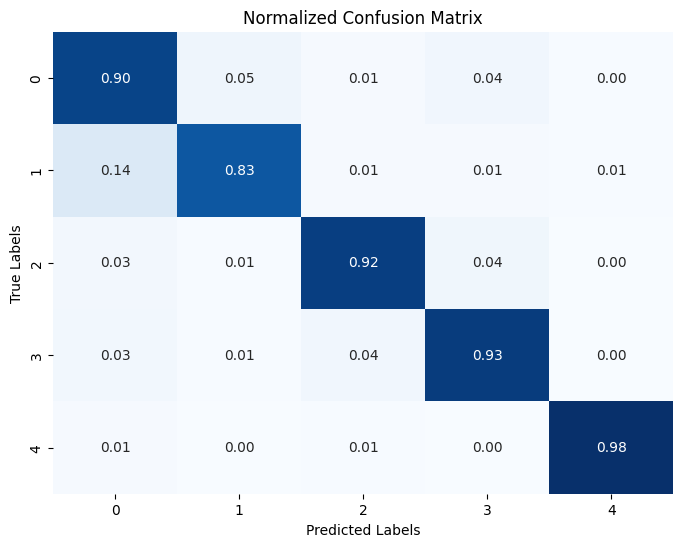
\includegraphics[width=0.4\linewidth]{figs/svc_crud.png}
    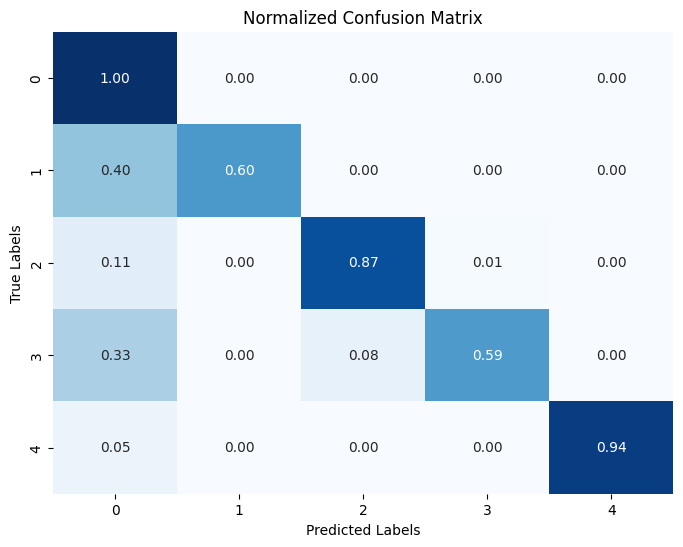
\includegraphics[width=0.4\linewidth]{figs/random_for_crud.png}
    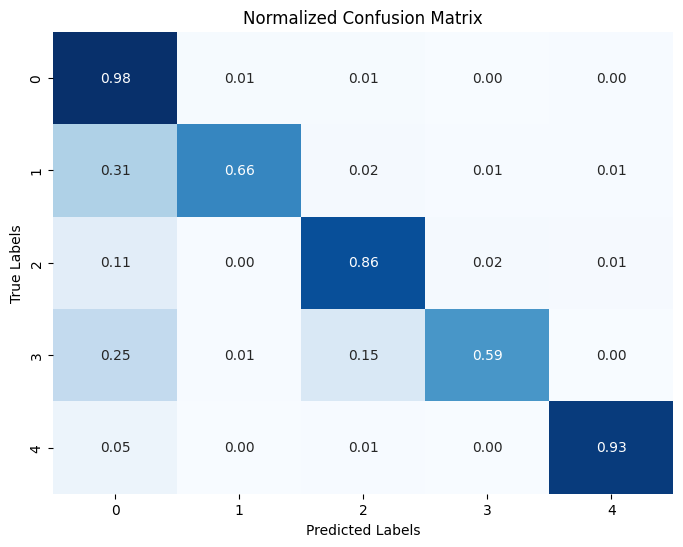
\includegraphics[width=0.4\linewidth]{figs/d_tree_crud.png}
    
    \caption{Without signal processing}
    \label{fig:crude_data}
\end{figure}

Following this foundational analysis, we implemented signal processing techniques to augment the dataset prior to classification. Specifically, we applied Fourier Transform decomposition and second derivative analysis to the raw data. These preprocessing steps yielded an accuracy score of 0.55 with an SVM, a 0.96 with an RFC, and a 0.94 with DTC; suggesting a significant reduction in categorization effectiveness compared to the baseline. The significant reduction in categorization effectiveness compared to the baseline suggests that the choice of preprocessing technique may not be universally beneficial across all machine learning algorithms. Results for the corresponding accuracies are presented in Figure 2.

\begin{figure}
    \centering
    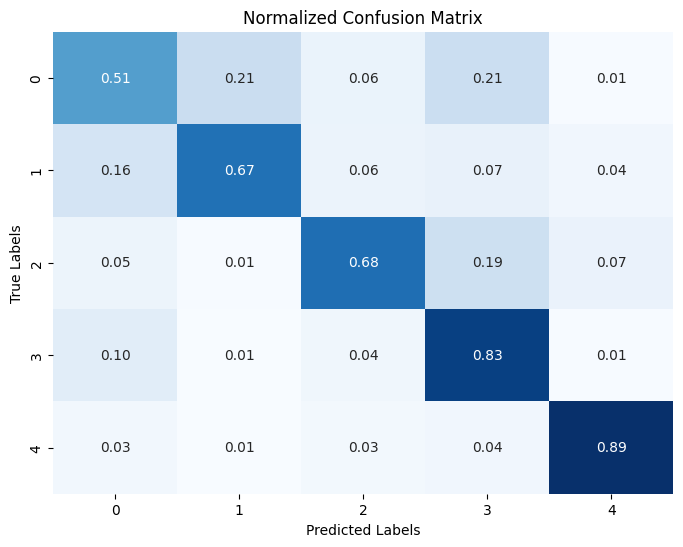
\includegraphics[width=0.4\linewidth]{figs/svc_processed.png}
    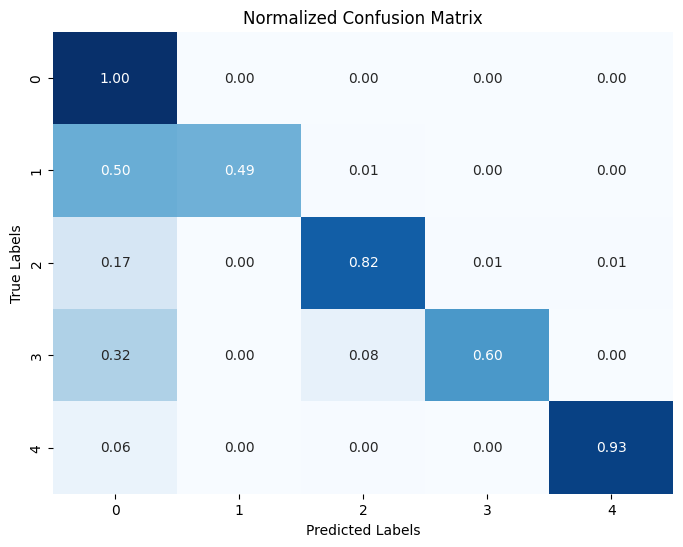
\includegraphics[width=0.4\linewidth]{figs/random_forest_processed.png}
    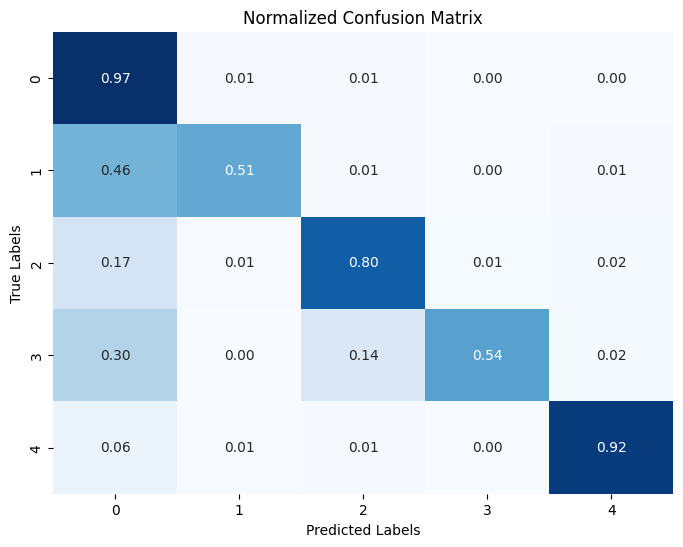
\includegraphics[width=0.4\linewidth]{figs/d_tree_processed.png}
    \caption{With signal processing}
    \label{fig:data_transformed}
\end{figure}

To mitigate the decline in accuracy observed after applying signal processing techniques, we explored alternative approaches. Our investigation revealed that segmenting the signal into 20 time intervals resulted in a substantial improvement in accuracy, achieving a score of 0.87 with an SVM, a 0.96 with a RFC, and a 0.94 with a DTC. This finding suggests that temporal segmentation of the ECG signals may enhance the machine learning models' ability to discern meaningful patterns within the data.Results for the corresponding accuracies are presented in Figure 3.
\begin{figure}
    \centering
    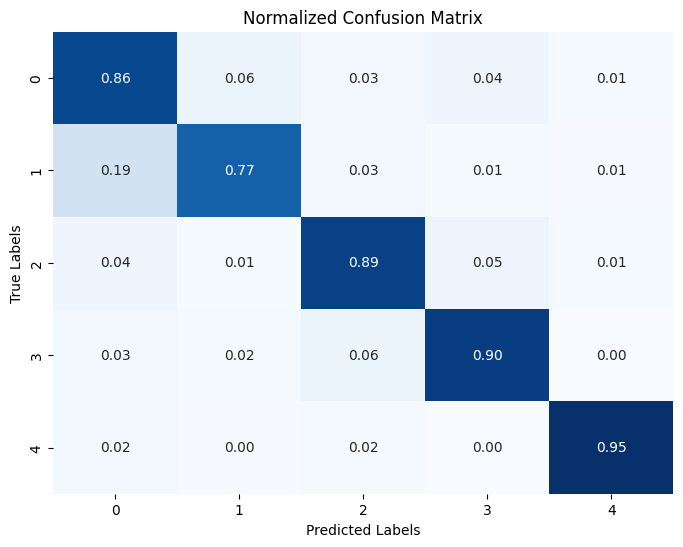
\includegraphics[width=0.4\linewidth]{figs/svc_proc2.png}
    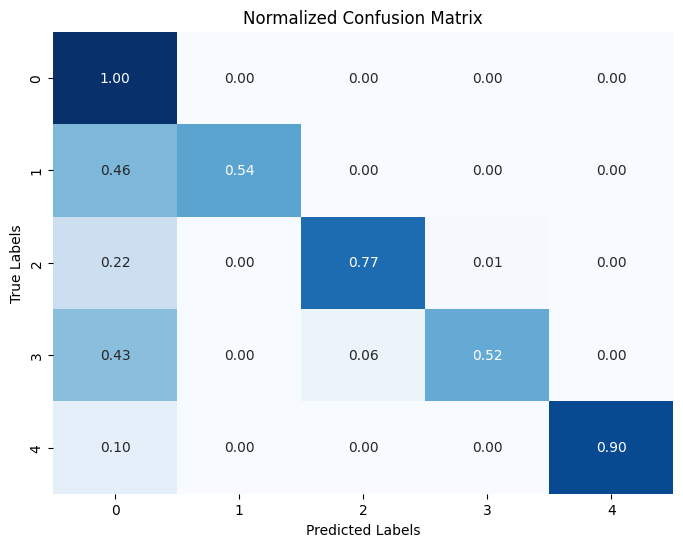
\includegraphics[width=0.4\linewidth]{figs/random_for_proc2.png}
    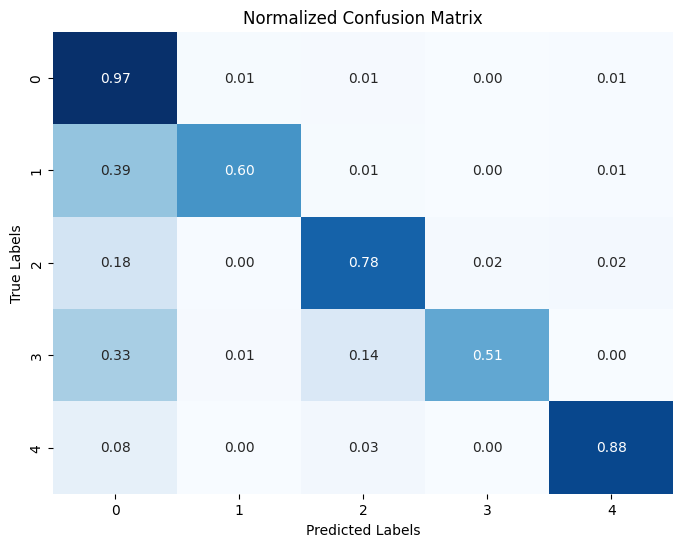
\includegraphics[width=0.4\linewidth]{figs/d_tree_proc2.png}
    \caption{With Signal processing and decomposition}
    \label{fig:data_segmented}
\end{figure}

Furthermore, we conducted an experiment involving the augmentation of the original dataset by appending the processed data. This approach led to an accuracy score of 0.88 with an SVM, a 0.97 with a RFC, and 0.95 with a DTC; demonstrating a moderate enhancement relative to the baseline performance. Results for the corresponding accuracies are presented in Figure 4.

\begin{figure}
    \centering
    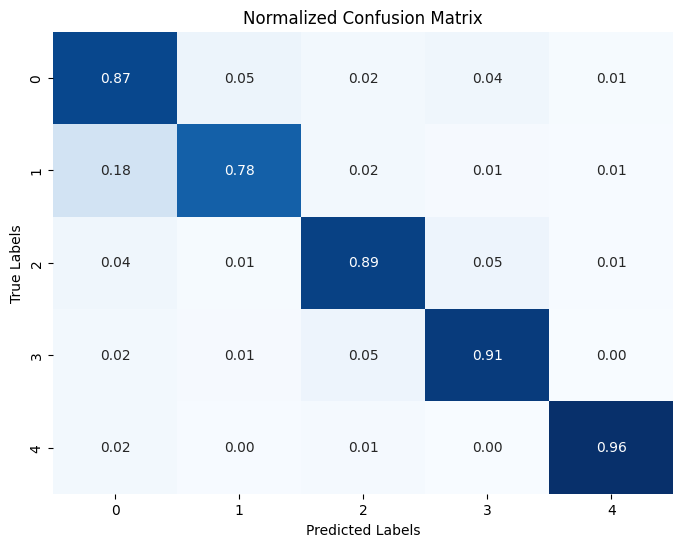
\includegraphics[width=0.4\linewidth]{figs/svc_proc_orig.png}
    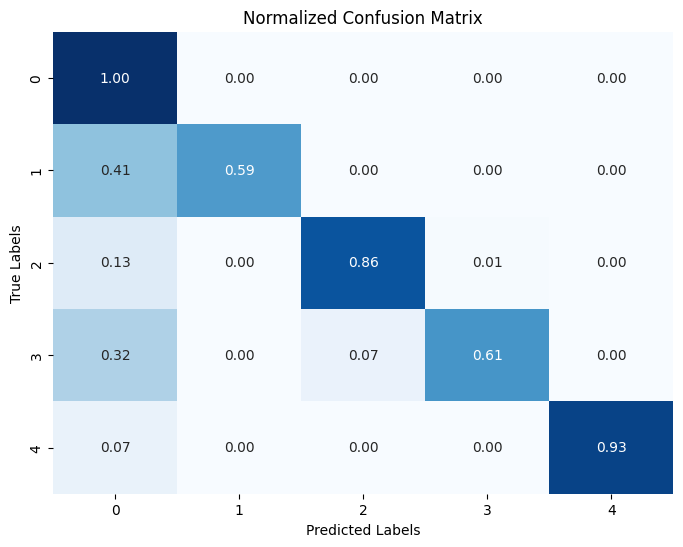
\includegraphics[width=0.4\linewidth]{figs/random_for_proc_orig.png}
    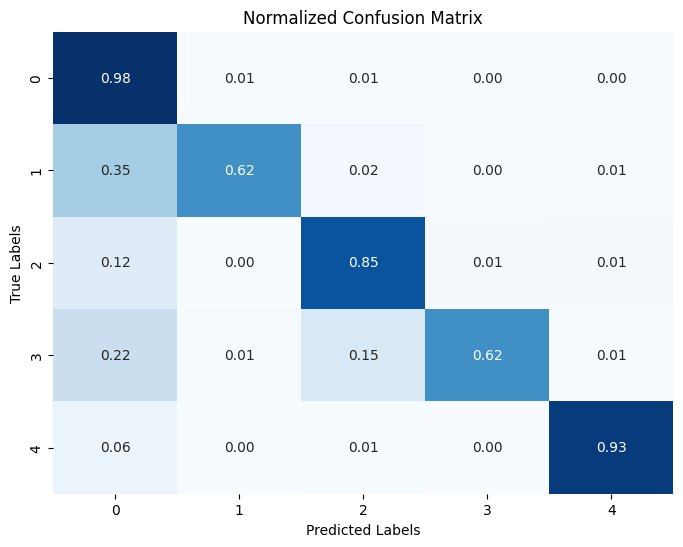
\includegraphics[width=0.4\linewidth]{figs/d_tree_proc_orig.png}
    \caption{Applied all transforms}
    \label{fig:mixed_data}
\end{figure}


\section{Conclusion}

These findings contribute to our understanding of the complex interplay between signal processing techniques, data segmentation, and machine learning algorithms in the context of ECG categorization. The varying degrees of success achieved through different preprocessing strategies underscore the importance of carefully considering the nature of the data and the specific characteristics of the machine learning models employed.

Future research endeavors might focus on optimizing the parameters of signal segmentation and exploring alternative preprocessing techniques to further enhance the accuracy of ECG categorization models. Additionally, comparative studies investigating the efficacy of various machine learning algorithms in conjunction with these preprocessing methods could provide valuable insights into the optimal approach for ECG signal analysis.


%
% ---- Bibliography ----
%
% BibTeX users should specify bibliography style 'splncs04'.
% References will then be sorted and formatted in the correct style.
%
% \bibliographystyle{splncs04}
% \bibliography{mybibliography}

\bibliographystyle{alpha}

\bibliography{bibliografia}

\end{document}